\section{Method}
\label{sec:method}

\subsection{Problem Setup}

Let $x$ be a prompt, $\pi_\theta$ be the student policy, and $\pi_T$ be a fixed teacher policy. The student samples a response
$y_i=(y_{i,1},\ldots,y_{i,T_i}) \sim \pi_\theta(\cdot \mid x)$.
For each response position $t$, we consider a candidate set
${\cal C}_{i,t}=\{a_{i,t,k}\}_{k=1}^{K}$. In the sampled-token setting, $K=1$ and $a_{i,t,1}=y_{i,t}$. In the top-$K$ setting, candidates may come from the student distribution, the teacher distribution, or their union.

On-policy distillation computes teacher and student log-probabilities on the same student-visited prefix:
\begin{equation}
\begin{aligned}
\ell^T_{i,t,k} =
\log \pi_T(a_{i,t,k}\mid x,y_{i,<t}),\\
\ell^\theta_{i,t,k} =
\log \pi_\theta(a_{i,t,k}\mid x,y_{i,<t}).
\end{aligned}
\end{equation}
The basic teacher-student log-probability gap is
\begin{equation}
\delta_{i,t,k} =
\ell^T_{i,t,k} - \ell^\theta_{i,t,k}.
\end{equation}
The dense OPD advantage can be written as
\begin{equation}
D_{i,t,k} = \rho_{i,t,k}\delta_{i,t,k},
\end{equation}
where $\rho_{i,t,k}$ is an optional candidate weight. For sampled-token OPD, $\rho_{i,t,k}=1$. Standard dense OPD directly uses
\begin{equation}
A^{\mathrm{OPD}}_{i,t,k}=D_{i,t,k}.
\end{equation}

Each sampled response also receives an outcome score $R_i$, provided by the task verifier. In our implementation this is the field \texttt{true\_reward\_score}. We convert it to a binary correctness label
\begin{equation}
c_i = {\bf 1}[R_i > 1/2],
\end{equation}
and a signed outcome label
\begin{equation}
z_i = 2c_i - 1.
\end{equation}
Thus $z_i=1$ for a correct response and $z_i=-1$ for an incorrect response.

\subsection{GRPO, OPD, and POV-OPD}

Figure~\ref{fig:pov_comparison} summarizes the difference between outcome-only RL, dense OPD, and POV-OPD. GRPO uses only the final outcome. Given a group of responses sampled for the same prompt, it computes a relative outcome advantage, for example
\begin{equation}
\hat R_i =
\frac{R_i-\mu(x_i)}{\sigma(x_i)+\epsilon},
\end{equation}
where $\mu(x_i)$ and $\sigma(x_i)$ are computed over responses to the same prompt. This scalar advantage is then broadcast to all response tokens:
\begin{equation}
A^{\mathrm{GRPO}}_{i,t} = \hat R_i.
\end{equation}
GRPO therefore gives reliable trajectory-level feedback, but it does not distinguish which local token decisions were useful.

OPD takes the opposite approach. It provides dense token-level teacher guidance on the student trajectory, but it does not check whether a local teacher preference is consistent with the final outcome. POV-OPD combines the two views. It keeps the dense OPD advantage $D_{i,t,k}$, but multiplies it by validation weights derived from the final outcome and from teacher prefix statistics:
\begin{equation}
A^{\mathrm{POV}}_{i,t,k}
=
D_{i,t,k}
\cdot
w^{\mathrm{out}}_{i,t,k}
\cdot
w^{\mathrm{pre}}_{i,t}
\cdot
b_{i,t,k}.
\end{equation}
Here $w^{\mathrm{out}}$ is the outcome-validation weight, $w^{\mathrm{pre}}$ is the prefix-validation weight, and $b$ is an aligned-candidate boost.

\begin{figure*}[t]
\centering
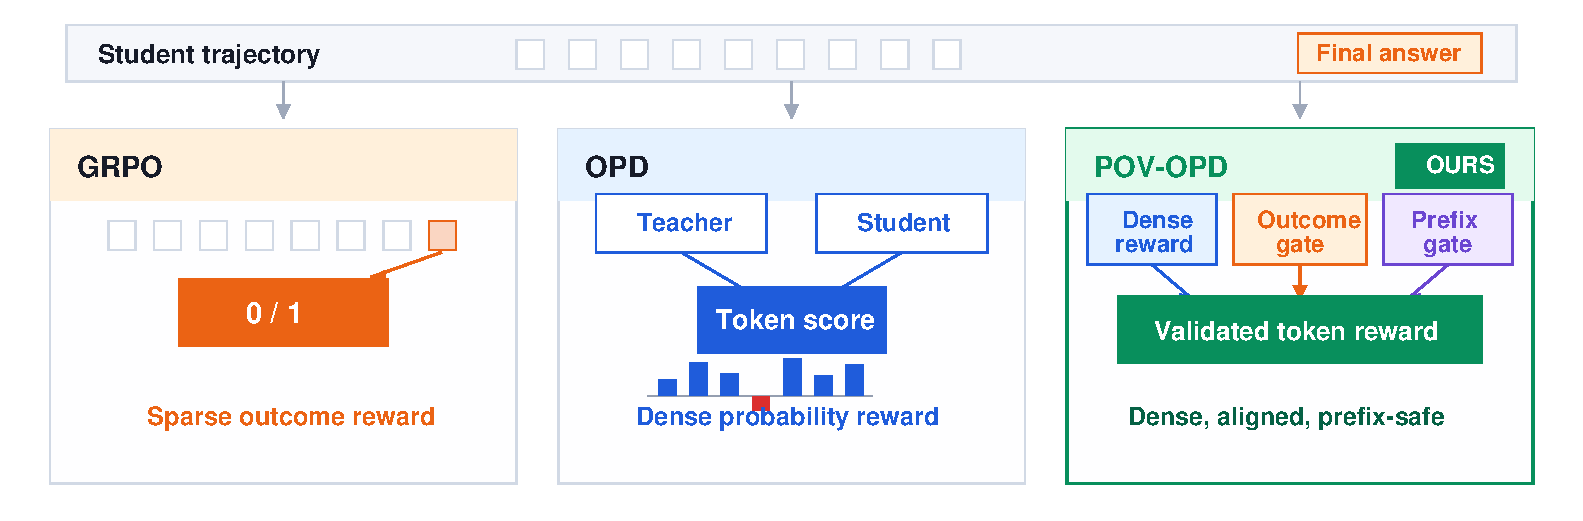
\includegraphics[width=\textwidth]{figures/pov_comparison.pdf}
\caption{Credit assignment on the same student rollout. GRPO group-normalizes the terminal verifier reward and broadcasts one scalar within each trajectory, whereas OPD provides signed dense teacher--student gaps without validating them. POV-OPD turns the terminal result into a local outcome-validity weight, detects sustained prefix drift from windowed teacher excess surprisal using CUSUM, and boosts only aligned candidates that remain well supported by the teacher. The sampled-token example at the bottom shows how the three nonnegative weights preserve, remove, cap, or decay each dense OPD signal without reversing its sign.}
\label{fig:pov_comparison}
\end{figure*}


\subsection{Outcome Validation}

Outcome validation checks whether the teacher-student preference points in the direction suggested by the final outcome. We use the alignment score
\begin{equation}
g_{i,t,k}=\delta_{i,t,k},
\end{equation}
and define the signed alignment score
\begin{equation}
s_{i,t,k}=z_i g_{i,t,k}.
\end{equation}
For a correct response, $z_i=1$, so a candidate is aligned when the teacher assigns it higher log-probability than the student. For an incorrect response, $z_i=-1$, so a candidate is aligned when the teacher assigns it lower log-probability than the student. With margin $m \geq 0$, the aligned and anti-aligned sets are
\begin{equation}
{\cal A}_i=\{(t,k):s_{i,t,k}>m\},
\quad
{\cal B}_i=\{(t,k):s_{i,t,k}<-m\}.
\end{equation}
Candidates with $|s_{i,t,k}|\leq m$ are treated as ambiguous.

The hard outcome-validation weight keeps only aligned candidates:
\begin{equation}
w^{\mathrm{out}}_{i,t,k}
=
{\bf 1}[(t,k)\in{\cal A}_i].
\end{equation}
This removes outcome-conflicting dense rewards, but it can be brittle when either the local teacher preference or the final verifier signal is noisy.

POV-OPD therefore also uses a rank variant. The rank variant preserves all aligned candidates at full weight and assigns only beta-capped weights to anti-aligned candidates. Let $n_i=|{\cal B}_i|$. For $(t,k)\in{\cal B}_i$, define
\begin{equation}
q_{i,t,k}
=
\left\{
\begin{array}{ll}
1, & n_i=1,\\
\frac{\mathrm{rank}_{{\cal B}_i}(s_{i,t,k})}{n_i-1}, & n_i>1.
\end{array}
\right.
\end{equation}
The lowest signed score in ${\cal B}_i$ has rank $0$, and the largest signed score in ${\cal B}_i$ has rank $n_i-1$. Thus anti-aligned candidates closer to the margin receive larger rank weights. With $\beta\in[0,1]$, the rank outcome-validation weight is
\begin{equation}
w^{\mathrm{out}}_{i,t,k}
=
\left\{
\begin{array}{ll}
1, & (t,k)\in{\cal A}_i,\\
\beta q_{i,t,k}, & (t,k)\in{\cal B}_i,\\
0, & |s_{i,t,k}|\leq m.
\end{array}
\right.
\end{equation}
This differs from globally reweighting all candidates: aligned candidates are not down-weighted, and $\beta$ only controls the maximum retained strength of anti-aligned supervision.

POV-OPD also supports position-level validation. Instead of validating each candidate separately, it first aggregates the alignment score at a position:
\begin{equation}
s_{i,t}^{\mathrm{pos}}
=
z_i\sum_{k=1}^{K} g_{i,t,k}.
\end{equation}
The hard position variant keeps positions with $s_{i,t}^{\mathrm{pos}}>m$. The rank position variant ranks only positions with $s_{i,t}^{\mathrm{pos}}<-m$, assigns them beta-capped weights, and broadcasts the resulting position weight to all candidates at that position. These variants test whether outcome consistency should be judged at the candidate level or at the next-token decision level.

\subsection{Prefix Validation}

Outcome validation checks the direction of local teacher preferences. Prefix validation checks whether the teacher remains reliable on the student-generated prefix. Let
\begin{equation}
H^T_{i,t}
=
-\sum_a \pi_T(a\mid x,y_{i,<t})
\log \pi_T(a\mid x,y_{i,<t})
\end{equation}
be the teacher entropy at position $t$. For the sampled token $y_{i,t}$, define teacher excess surprisal
\begin{equation}
u_{i,t}
=
-\log \pi_T(y_{i,t}\mid x,y_{i,<t})
-
H^T_{i,t}.
\end{equation}
A positive value means that the sampled token is more surprising under the teacher than a typical token drawn from the teacher distribution at the same prefix.

For each response, we divide valid response tokens into consecutive windows of size $W$. Let $\bar u_{i,b}$ be the mean excess surprisal in window $b$. The first $L$ windows form a baseline, with
\begin{equation}
\mu_i =
\frac{1}{L_i}\sum_{b=1}^{L_i}\bar u_{i,b},
\quad
L_i=\min(L,M_i),
\end{equation}
where $M_i$ is the number of windows in response $i$. For later windows, we compute relative excess
\begin{equation}
d_{i,b}=\bar u_{i,b}-\mu_i,
\end{equation}
and a one-sided CUSUM statistic
\begin{equation}
C_{i,b}
=
\max(0, C_{i,b-1}+d_{i,b}-\kappa),
\quad b>L_i,
\end{equation}
where $\kappa\geq 0$ is a drift allowance. The prefix horizon is the first post-baseline window whose CUSUM exceeds threshold $\tau$:
\begin{equation}
b_i^\star =
\min\{b>L_i:C_{i,b}>\tau\}.
\end{equation}
If no such window exists, all prefix weights remain one.

After the horizon is triggered, POV-OPD monotonically decays the prefix weight:
\begin{equation}
\begin{aligned}
\eta_{i,b} &=
\exp[-\lambda\max(C_{i,b}-\tau,0)],\\
w^{\mathrm{pre}}_{i,b}
&=
\left\{
\begin{array}{ll}
1, & b < b_i^\star,\\
\min(w^{\mathrm{pre}}_{i,b-1},\eta_{i,b}),
& b \geq b_i^\star .
\end{array}
\right.
\end{aligned}
\end{equation}
The token-level prefix weight $w^{\mathrm{pre}}_{i,t}$ is obtained by assigning the window weight to every valid token in that window. This produces a non-increasing trust weight after sustained teacher-surprisal drift.

\subsection{Aligned-Candidate Support}

POV-OPD gives a small boost to aligned candidates that are also well supported by the teacher distribution. For a candidate $a_{i,t,k}$, define
\begin{equation}
r_{i,t,k}
=
-\ell^T_{i,t,k}-H^T_{i,t}.
\end{equation}
The candidate support is
\begin{equation}
p^{\mathrm{sup}}_{i,t,k}
=
\exp[-\max(r_{i,t,k},0)].
\end{equation}
This support equals one when the candidate is no more surprising than the teacher entropy and decays when the candidate is unusually surprising under the teacher. The aligned boost is
\begin{equation}
b_{i,t,k}
=
1+\alpha p^{\mathrm{sup}}_{i,t,k}
{\bf 1}[(t,k)\in{\cal A}_i],
\end{equation}
where $\alpha\geq 0$ controls the boost strength. Anti-aligned and ambiguous candidates are not boosted.

\subsection{Final Objective}

The final POV-OPD advantage is
\begin{equation}
A^{\mathrm{POV}}_{i,t,k}
=
D_{i,t,k}
\cdot
w^{\mathrm{out}}_{i,t,k}
\cdot
w^{\mathrm{pre}}_{i,t}
\cdot
b_{i,t,k}.
\end{equation}
For sampled-token OPD, this expression reduces to $K=1$. For top-$K$ OPD, it applies to each candidate token.

The policy is optimized with the same PPO-style update used by OPD. Let
\begin{equation}
r_{i,t,k}(\theta)
=
\frac{\pi_\theta(a_{i,t,k}\mid x,y_{i,<t})}
{\pi_{\theta_{\mathrm{old}}}(a_{i,t,k}\mid x,y_{i,<t})}.
\end{equation}
Let $\bar r_{i,t,k}(\theta)=
\mathrm{clip}(r_{i,t,k}(\theta),1-\epsilon,1+\epsilon)$.
The clipped objective is
\begin{equation}
{\cal L}_{\mathrm{POV}}
=
-\sum_{i,t,k}
\min
\left(
r_{i,t,k}(\theta)A^{\mathrm{POV}}_{i,t,k},
\bar r_{i,t,k}(\theta)A^{\mathrm{POV}}_{i,t,k}
\right).
\end{equation}
POV-OPD therefore changes the credit assignment used to form advantages, while leaving rollout generation, teacher scoring, and the actor optimization pipeline unchanged.
